\documentclass{article}
\usepackage{graphicx}
\usepackage{subcaption}
\usepackage[table]{xcolor}
\usepackage{siunitx} % Required for alignment
\sisetup{
	round-mode      =places, % Rounds numbers
	round-precision  = 3, % to 2 places
}


\title{GST 108:Introduction to Quantitative Reasoning}
\author{Nkechi Grace Okoacha}
	
\begin{document}
		\textbf{\underline{LOGIC GATES}}
	
	A logic gate is a building block of a digital circuit which is at the heart of any computer operation
	
	
\begin{figure}
	\centering
	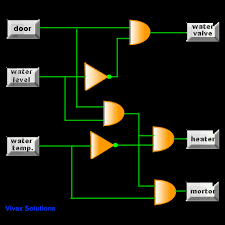
\includegraphics[width=\linewidth]{t}
	\caption{logic}
		\end{figure}
	
	Behind every digital system is a logic gate
	
	\begin{figure}
		\centering
		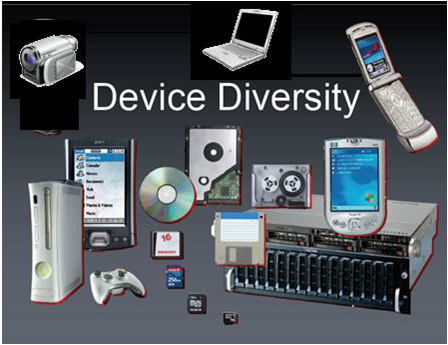
\includegraphics[width=\linewidth]{Picture 2}
		\caption{logic}
	\end{figure}

		\begin{itemize}
			\item Logic gates perform logical operations that take binary input (0s and 1s) and produce  a single binary output. They are used in most electronic device including
			
		\end{itemize}
	
	\newpage
	
	\begin{figure}[h!]
		\centering
		\begin{subfigure}[b]{0.2\linewidth}
			
			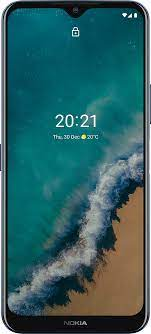
\includegraphics[width=\linewidth]{smartphone 1}
			\caption{device}\end{subfigure}
		\begin{subfigure}[b]{0.2\linewidth}
			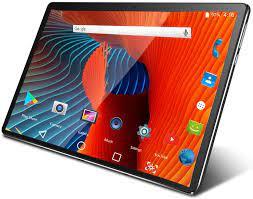
\includegraphics[width=\linewidth]{tab}
			\caption{tablet}
		\end{subfigure}
		\begin{subfigure}[b]{0.2\linewidth}
			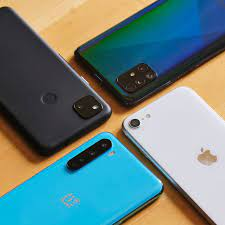
\includegraphics[width=\linewidth]{sm}
			\caption{phone}
		\end{subfigure}

	
	\end{figure}

Now think of a logic gate like a light switch, it is either in an ON or OFF position. Similarly, the input output terminals are always in one of two binary positions false(0) and true(1). Each gate has its own logic or set of rules that determines how it acts based on multiple inputs outlined in a truth table.

Combining 10s, 1000s or millions of logic gates makes it possible for a computer to perform highly complex operations and tasks at ever increasing speeds.

A gate is a basic electronic circuit which operates on one or more signals to produce an output signal. 
Logic gates are digital circuits constructed from diodes, transistors, and resistors connected in such a way that the circuit output is the result of a basic logic operation (OR, AND, NOT) performed on the inputs.

\textbf{\underline{TYPES OF LOGIC GATES}}

Fundamental gates are AND, OR and NOT

\begin{figure}[h!]
	\centering
	\begin{subfigure}[b]{0.2\linewidth}
		
		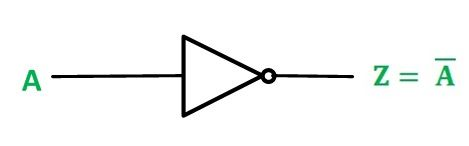
\includegraphics[width=\linewidth]{not}
		\caption{not gate}\end{subfigure}
	\begin{subfigure}[b]{0.2\linewidth}
		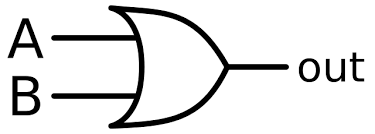
\includegraphics[width=\linewidth]{or}
		\caption{or gate}
	\end{subfigure}
	\begin{subfigure}[b]{0.2\linewidth}
		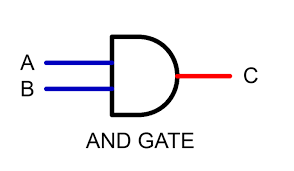
\includegraphics[width=\linewidth]{and}
		\caption{and gate}
	\end{subfigure}
\end{figure}
Derived Gates are NAND, NOR, XOR and XNOR (derived from the fundamental gates)

Universal Gates are NAND and NOR gates (the fundamental logic gates can be realized through them).

The expression C = A X B reads as “C equals A AND B“ 
The multiplication sign (X) stands for the AND operation, same for ordinary multiplication of 1s and 0s.


\begin{figure}[h!]
	\centering
	\begin{subfigure}[b]{0.2\linewidth}
		
		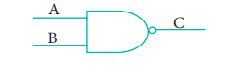
\includegraphics[width=\linewidth]{Picture 16}
		\caption{and}
	\end{subfigure}
	\end{figure}
The AND operation produces a true output (result of 1) only for the single case when all of the input variables are 1 and a false output (result of 0) where one or more inputs are 0.

\begin{table}[h!]
	\begin{center}
		\begin{tabular}{l|S|r|c|} % <-- Change to S here.
			\hline
			\cellcolor{red!35}\textbf{A} & \cellcolor{red!35}\textbf{B} & \cellcolor{red!35}\textbf{C= A X B}\\
			\hline
			\cellcolor{blue!35}1 & 1 & 1\\
			\cellcolor{blue!25}1 & 0 & 0\\
			\cellcolor{blue!25}0 & 1 & 0 \\
			\cellcolor{blue!25}0 & 0 & 0 \\
		\hline
		
	\end{tabular}
\end{center}
\end{table}

\begin{figure}
	\centering
	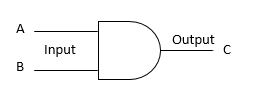
\includegraphics[width=\linewidth]{andd}
	\caption{AND GATE}
\end{figure}

The expression C = A + B reads as “C equals A OR B". It is the inclusive “OR”
The Addition (+) sign stands for the OR operation

\begin{figure}[h!]
	\centering
	\begin{subfigure}[b]{0.2\linewidth}
		
		
\includegraphics[width=\linewidth]{o}
		\caption{or gate}\end{subfigure}
	\end{figure}


	\end{document}